\documentclass[10pt,twocolumn,letterpaper]{article}

\usepackage{cvpr}
\usepackage{times}
\usepackage{epsfig}
\usepackage{graphicx}
\usepackage{amsmath}
\usepackage{amssymb}

% Include other packages here, before hyperref.

% If you comment hyperref and then uncomment it, you should delete
% egpaper.aux before re-running latex.  (Or just hit 'q' on the first latex
% run, let it finish, and you should be clear).
\usepackage[breaklinks=true,bookmarks=false]{hyperref}

\cvprfinalcopy % *** Uncomment this line for the final submission

\def\cvprPaperID{****} % *** Enter the CVPR Paper ID here
\def\httilde{\mbox{\tt\raisebox{-.5ex}{\symbol{126}}}}

% Pages are numbered in submission mode, and unnumbered in camera-ready
%\ifcvprfinal\pagestyle{empty}\fi
\setcounter{page}{4321}
\begin{document}

%%%%%%%%% TITLE
\title{Dynamic Locomotion Terrain Recognition for the MIT Cheetah 3 Robot \\ 6.869 / 6.819: Advances in Computer Vision}

\author{Gerardo Bledt\\
Massachusetts Institute of Technology\\
Cambridge, MA\\
{\tt\small gbledt@mit.edu, 6.869}
% For a paper whose authors are all at the same institution,
% omit the following lines up until the closing ``}''.
% Additional authors and addresses can be added with ``\and'',
% just like the second author.
% To save space, use either the email address or home page, not both
\and
Milo Knowles\\
Massachusetts Institute of Technology\\
Cambridge, MA\\
{\tt\small mknowles@mit.edu, 6.819}
}

\maketitle
%\thispagestyle{empty}

%%%%%%%%% ABSTRACT
\begin{abstract}
   Our goal in this project is to create an inexpensive, lightweight and robust vision system that can estimate the terrain in front of the MIT Cheetah 3 robot in real time. Using a stereo rig consisting of two \$20 webcams, we are able to obtain metrically accurate 3D reconstructions of planar obstacles from image pairs. In addition, by fitting a polytope to noisy terrain point clouds, our representation of the terrain is robust to outliers and has a very compact parametrization. This allows real time communication of the sensed enfironment to the robot, which allows it to modify its trajectory plan according to the vision input.
\end{abstract}

%%%%%%%%% BODY TEXT

%!TEX root = ../egpaper_final.tex

\section{Introduction}

Currently, the MIT Cheetah 3 robot uses primarily completely blind locomotion. What this means is that there is no vision or LiDAR system that allows it to preemptively sense its environment or plan for upcoming obstacles. Dynamic gaits such as trotting have been stabilized under ideal flat-terrain conditions, but most interesting applications of robotics involve some kind of unstructured, non-flat, non-smooth terrain situations. Recent research efforts have allowed for reactive tactile environment sensing where the robot is able to interpret and build its knowledge of the environment when it senses unexpected contact with a surface \cite{Bledt2018}. This has allowed for the same nominal dynamic gaits to stabilize in rough terrains by reacting to the estimated foot contacts. 

However, since this environment sensing is purely reactionary, the robot can only detect objects and uneven ground after it has already determined contact with the surface. This covers a lot of cases where small objects and holes are littered over terrain with a slowly changing gradient. A current challenge is when the robot encounters a large, sharp terrain disturbances, such as a box or a set of stairs, it will not be able to smoothly use this reactionary sensing to navigate the terrain. If the box or stair is higher than the nominal foot swinging height as it is in Figure \ref{fig:RI}, it will simply not be able to step over it and will not detect a support surface contact when it does hit the side. Similarly, if the box or stair is higher than its possible foot swing height, it will not be able to continue forward and crash. By incorporating some visual terrain recognition, the robot will be able to modify its swing foot trajectory to clear objects that are within its kinematic workspace, as well as feed terrain information to the contact detection algorithm for more accurate probabilistic ground height models.

\begin{figure}[t]
\centering
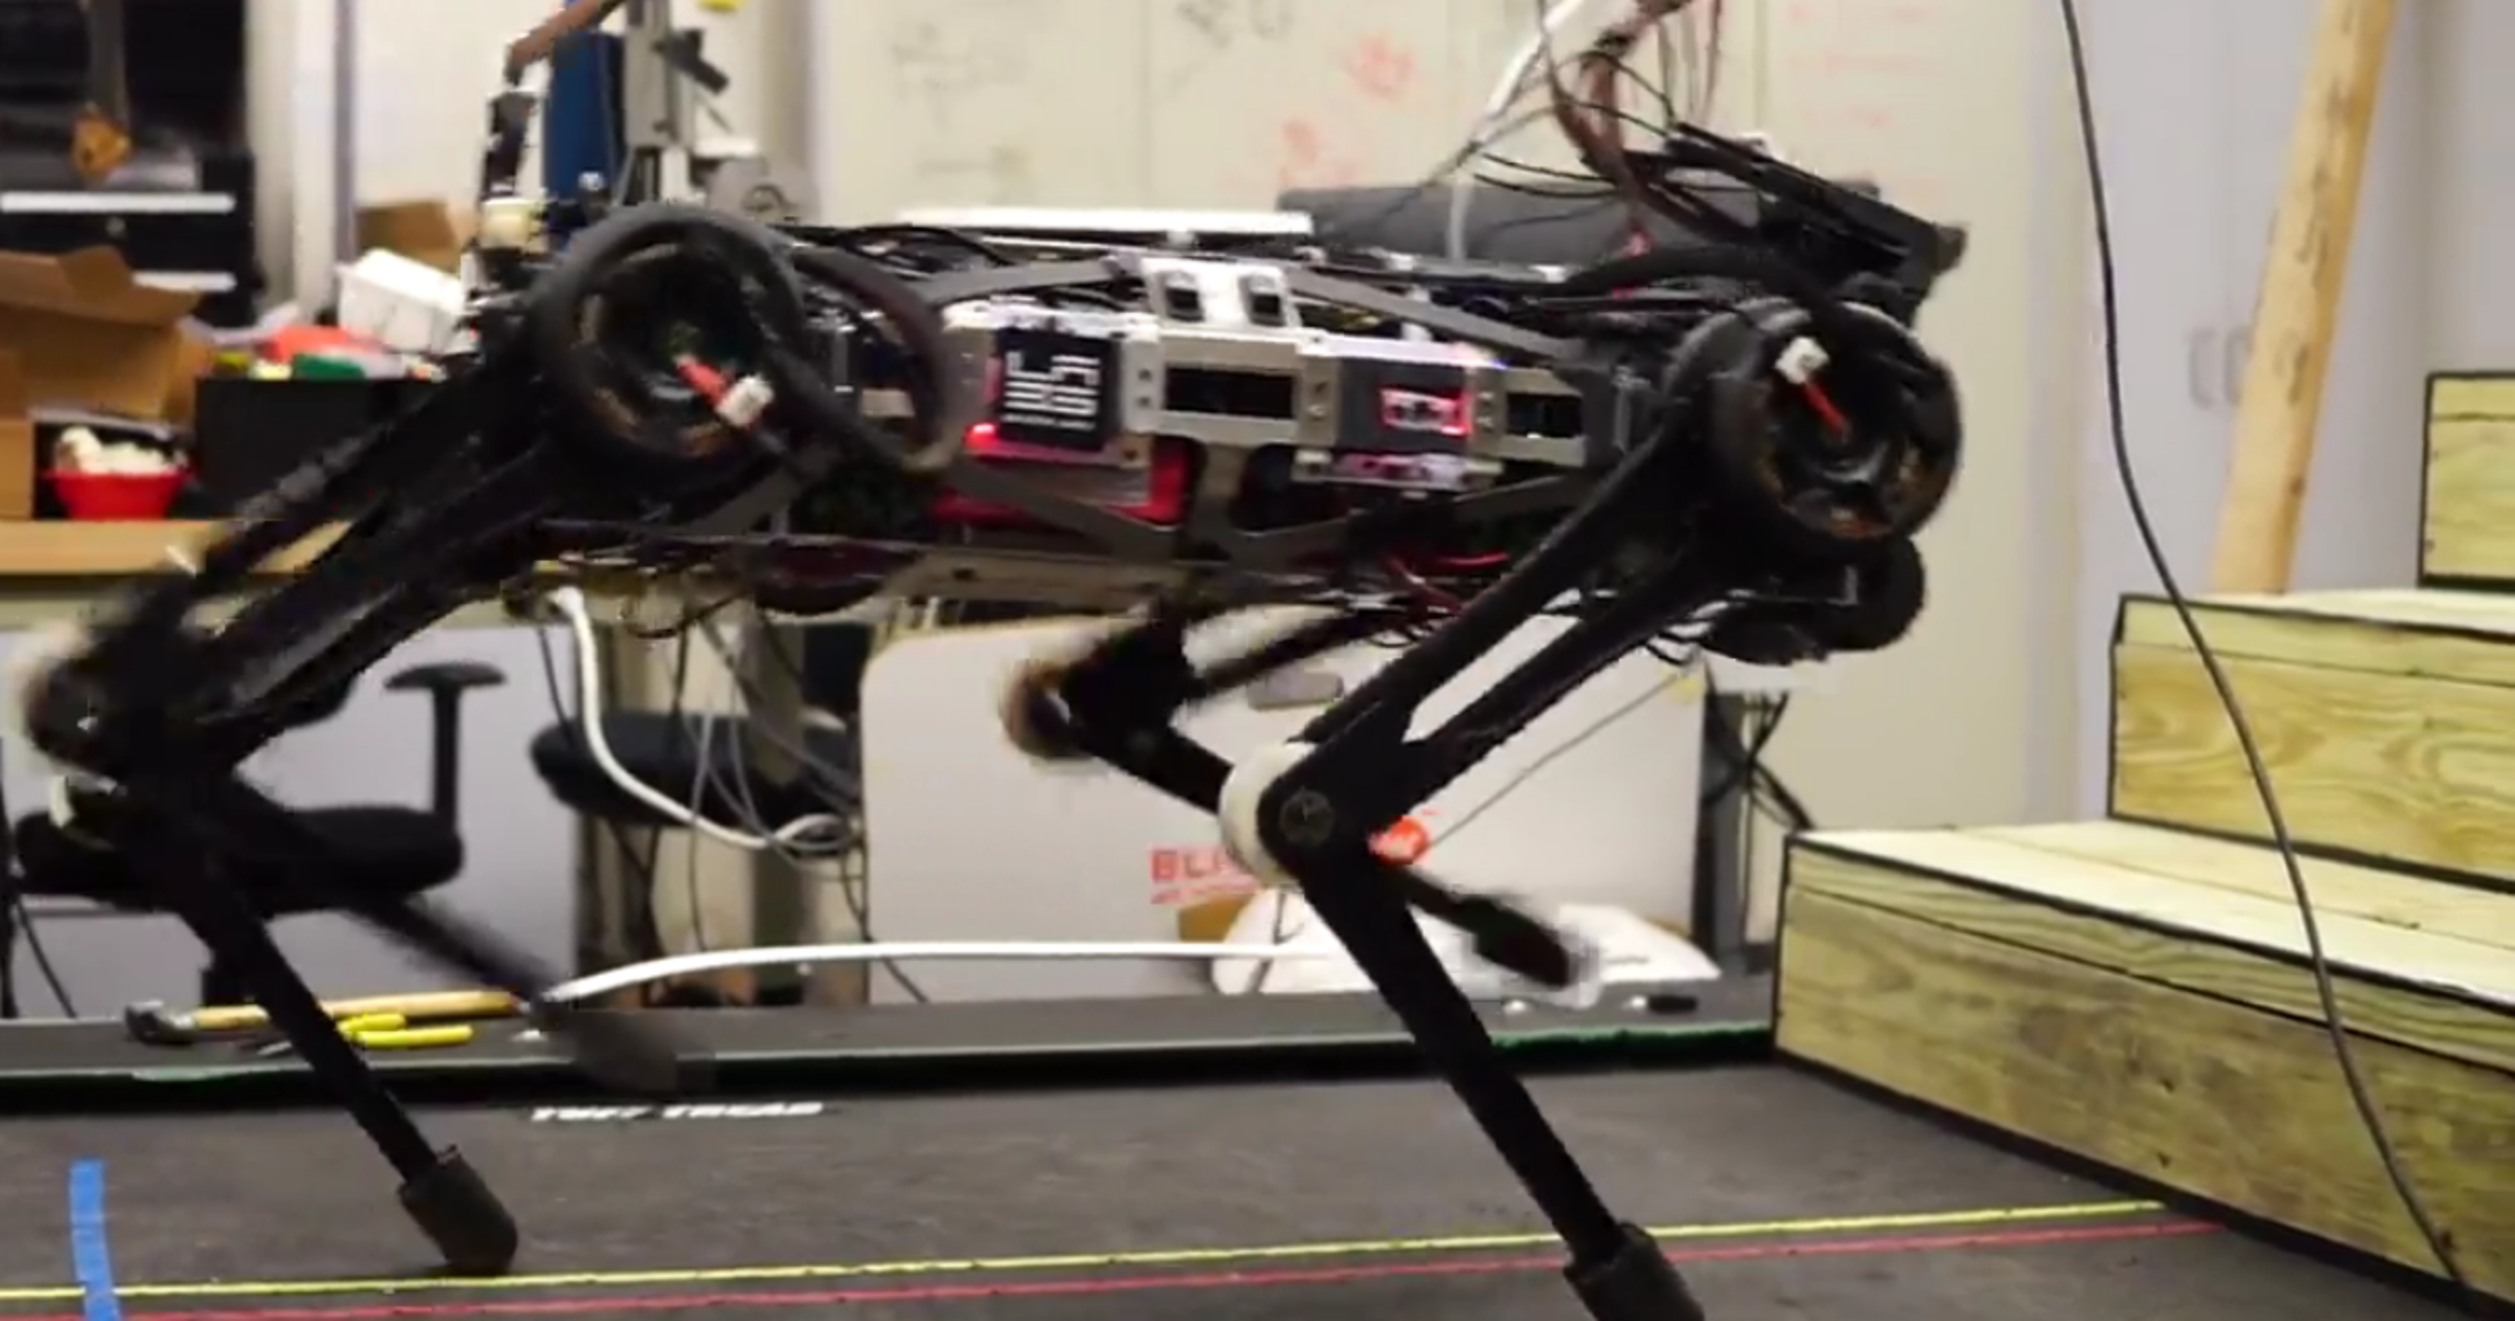
\includegraphics[width=\columnwidth]{Figures/RobotIntro.pdf}
\caption{A robust controller is used for general robot locomotion in unstructured terrains, but a method of external environment sensing is needed for the robot to know that its nominal foot swing trajectory will not be able to clear the stair obstacle.}
\label{fig:RI}
\end{figure}

Paper on creating the disparity map \cite{1467526} 

%!TEX root = ../egpaper_final.tex

\section{Related Work}

%!TEX root = ../egpaper_final.tex
\section{Approach}

Our pipeline is summarized in Figure \ref{overview-diagram}. We begin with a pair of RGB stereo images. From this image pair and calibration parameters obtained offline, we apply a stereo matching algorithm (See Section \ref{stereo-matching-section} to get a depthmap of the scene. Using camera instrinsic parameters, we can project this depthmap into 3D space and obtain a point cloud of the environment (See Section \ref{pointcloud-section}). Using two different methods described in Section \ref{plane-section}, we decompose this point coud into a set of planes. Finally, we reconstruct a polytope from these planes. A robot can use this geometric representation of the terrain to plan its foot trajectory.


\begin{figure}[!h]
\centering
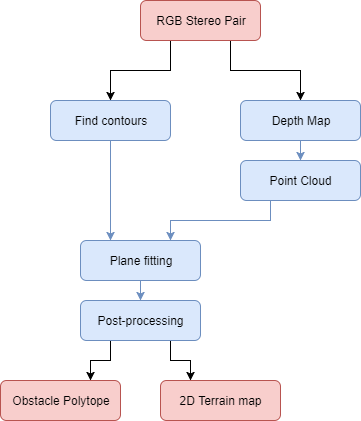
\includegraphics[width=2in]{Sections/Figures/Final-Project-Pipeline.png}
\caption{An overview of our obstacle reconstruction pipeline.}
\label{overview-diagram}
\end{figure}

\subsection{Stereo Matching for 3D Pointcloud} \label{stereo-matching-section}
The goal for stereo vision is to take two separate pictures of the same scene from two cameras at known relative distances and orientations form each other and attempt to reconstruct the 3D version of the scene. This is the general principle behind the human vision system that has depth perception. In our experiment we set two parallel cameras about 8 cm apart in the same direction which results in pictures like the one in Figure \ref{stereo-image-pair}.
\begin{figure}[!h]
\centering
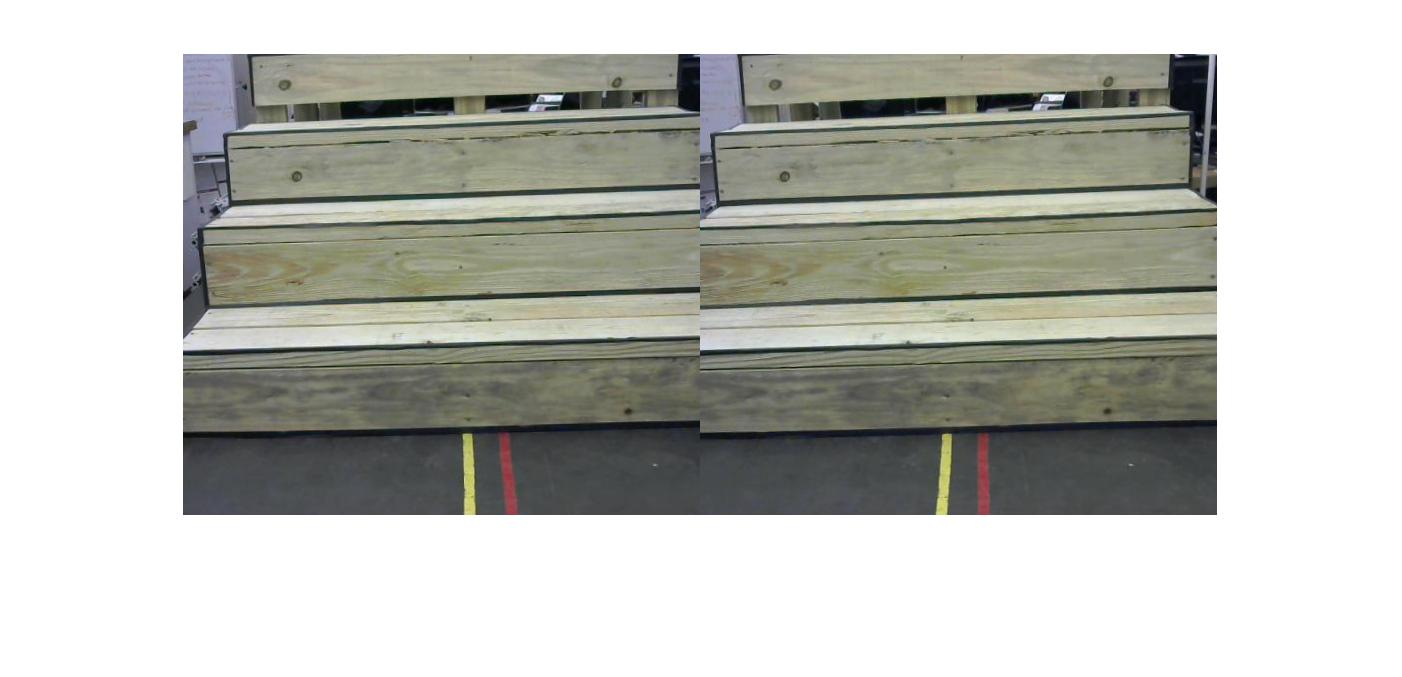
\includegraphics[width=3.3in]{Sections/Figures/example_stereo_pair.jpg}
\caption{Am image pair taken by our stereo camera setup. The two cameras are parallel and have a baseline of approximately 8cm.}
\label{stereo-image-pair}
\end{figure}

\begin{figure}[!h]
\centering
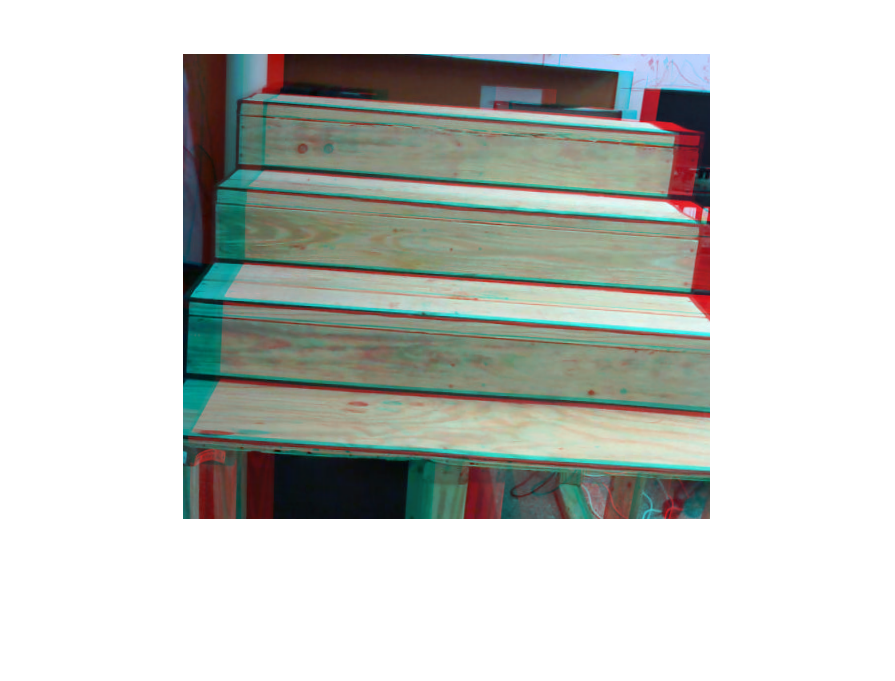
\includegraphics[width=3.3in]{Sections/Figures/stereo_anaglyph.png}
\caption{An example stereo anaglyph.}
\label{stereo-anaglyph}
\end{figure}

In order to find the best match between the two images, we used a technique called Semi-Global Matching as described in \cite{1467526}. The basic premise follows an optimization that compares the two images with a matching cost defined by the following cost function
\begin{align*}
E(D) = \sum\limits_p(C(p,D_p)+\sum\limits_{q\in N_p}P_1T[|D_p-D_q|=1]+\\\sum\limits_{q\in N_p}P_2T[|D_p-D_q|>1])
\end{align*}
Here, the optimization travels along many paths throughout the image and the costs from each path are summed and the lowest cost disparity is chosen for each pixel. The cost function has the first term being the sum of the pixel matching costs for the disparities, the second term being a penalty for 1 pixel disparity, and the third being a large cost for bigger pixel disparities.

The method results in a disparity image that gives the estimated depth to each pixel. This disparity is then used to create a 3D representation of the scene since we know the depth at each 2D pixel. This results in a pointcloud with $Z$ being the distance from the camera locations. The original image in then overlaid onto the pointcloud as seen in Figure \ref{pointcloud-example}. Although the pointcloud is not an exact representation of the actual scene, many post-processing steps were taken to smooth out the noise and extract features from the pointcloud.
\begin{figure}[!h]
\centering
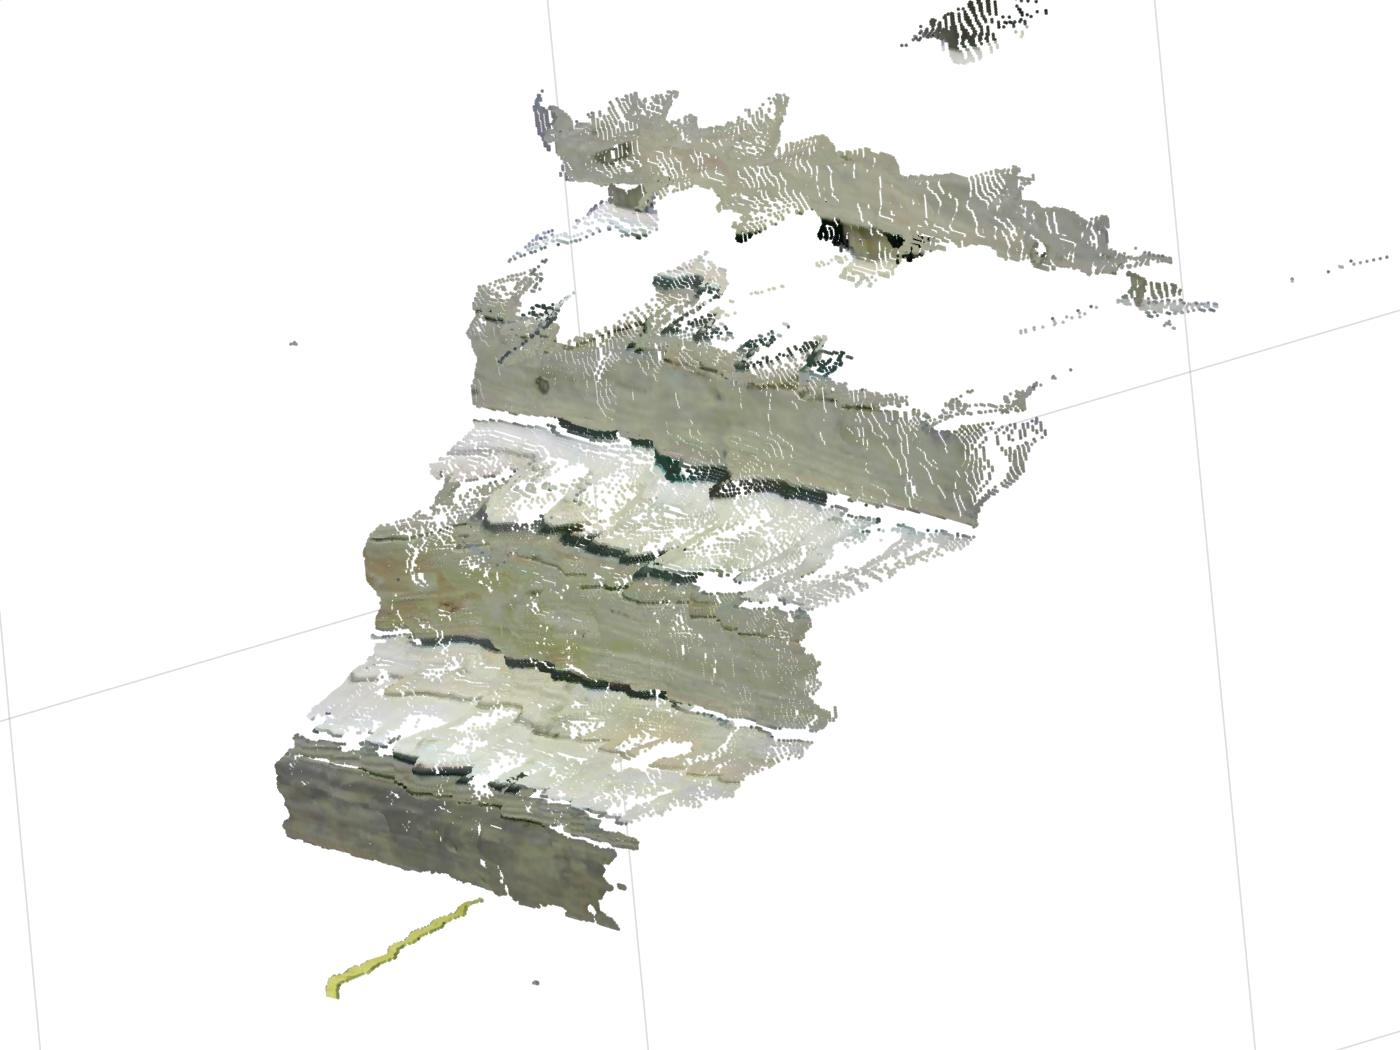
\includegraphics[width=3.3in]{Sections/Figures/example_stairs_pointcloud.jpg}
\caption{A pointcloud representation of the stairs in Figure \ref{stereo-image-pair}.}
\label{pointcloud-example}
\end{figure}

\subsection{Planar Decomposition of Point Clouds} \label{plane-section}

In order to estimate a polytope representation of an obstacle, decompose its point cloud into a set of planes. We demonstrate two main approaches for finding planar surfaces of an obstacle. We describe the Contour Method in Section \ref{contour-method} and the Orientation Method in \ref{orient-method}.

Each method has its advantages and limitations. While the Contour Method can generalize to planar surfaces with arbitary orientation, it is highly sensitive to the texture and edges of obstacles. The Orientation Method is more robust to appearance, but is limited to vertical and horizontal planes.

In both approaches, MSAC (M-Estimator SAmple Consensus \cite{msac-article}) is the algorithm used for plane estimation. In \cite{msac-article}, Zisserman et. al. show that MSAC is more robust than RANSAC for estimating geometric relationships in point cloud data, at no additional computational cost.

\subsubsection{Contour Method} \label{contour-method}

As the name of this approach suggests, we detect large contours in the original RGB image and project these contours into the point cloud to find subsets points that are likely to be coplanar.

We use MATLAB's \textit{imcontour} function from the Computer Vision Toolkit to efficiently find contours. Internally, this function uses the Theo Pavlidis algorithm \cite{pavlidis} to find contours at a variable number of levels.

Contours are then sorted by area, and pairs of contours with Intersection-over-Union (IoU) above a threshold of 0.3 are replaced by the larger of the two contours. Highly overlapping contours are likely to lie on the same plane, and we observe empirically that our reconstruction performs better when there are no duplicate planes.

We then project our candidate contours into the point cloud, and find 3D points that originally from inside of this contour in the RGB image. A plane is fit to each planar subset of the point cloud using MSAC.

\begin{figure}[!h]
\centering
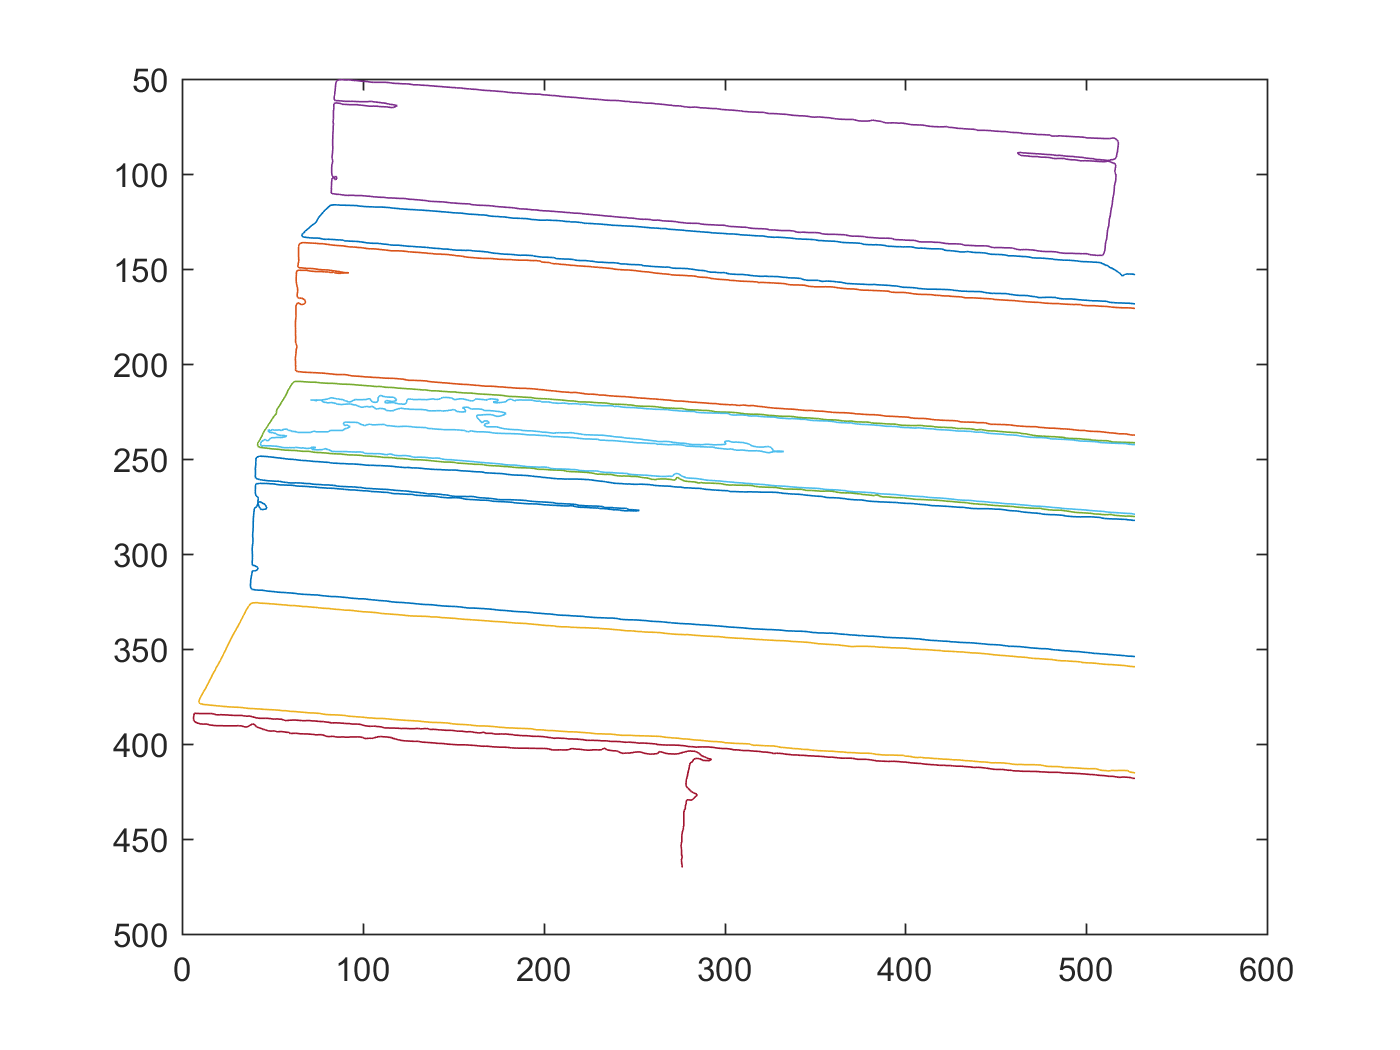
\includegraphics[width=3.3in]{Sections/Figures/good_contour_plot_12-7.png}
\caption{An example contour plot of the stairs in Figure \ref{stereo-anaglyph}. Here we have shown the eight largest contours in the image by area.}
\label{contours-example}
\end{figure}

\subsubsection{Orientation Method} \label{orient-method}

The Contour Method, as one might expect, is highly sensitive to lighting effects and the sharpness of edges on the obstacle. In this section, we propose a second method that relies on \textit{au priori} knowledge of plane orientation to remove our dependence on image contours.

In this method, we assume that the obstacle is composed of a predetermined number of planes that are either horizontal and vertical relative to the world frame. While performing MSAC, we sample three points from the point cloud and compute the parameters of a plane with them. We require that the normal of this plane is within an angular tolerance of a reference normal vector (i.e the z-axis for vertical planes and the y-axis for horizontal planes). If the robot frame is not aligned with the world frame, we can rotate our reference normals before performing MSAC. After performing a fixed number of iterations, MSAC selects a horizontal or vertical plane with the lowest cost. We then remove the inlier points from the point cloud, and iteratively fit horizontal and vertical planes to the residual point cloud.

Although our algorithm currently looks for a fixed number of planes, it would be straightforward to add a condition that stops extracting planes once the residual point cloud is too small, or the cost of MSAC planes is above a threshold.

\subsection{Polytope Reconstruction from Unordered Planes} \label{polytope-section}

At this stage in the pipeline, we have an unordered set of planes, each represented by four parameters: a surface normal and offset constant. There are many ways that these planes could intersect to form a polytope, but only one that actually matches our ground truth observation. We must make another assumption here about the composition of the polytope.

When using the Contour Method in Section \ref{contour-method}, we assume that the depth and height ordering of planes in 3D space is given by the vertical ordering of planes in the RGB image. Horizontal planes that appear higher in the RGB image are also higher in the scene. Similarly, vertical planes that appear higher in the RGB image are deeper in the scene.

\begin{figure}[!h]
\centering
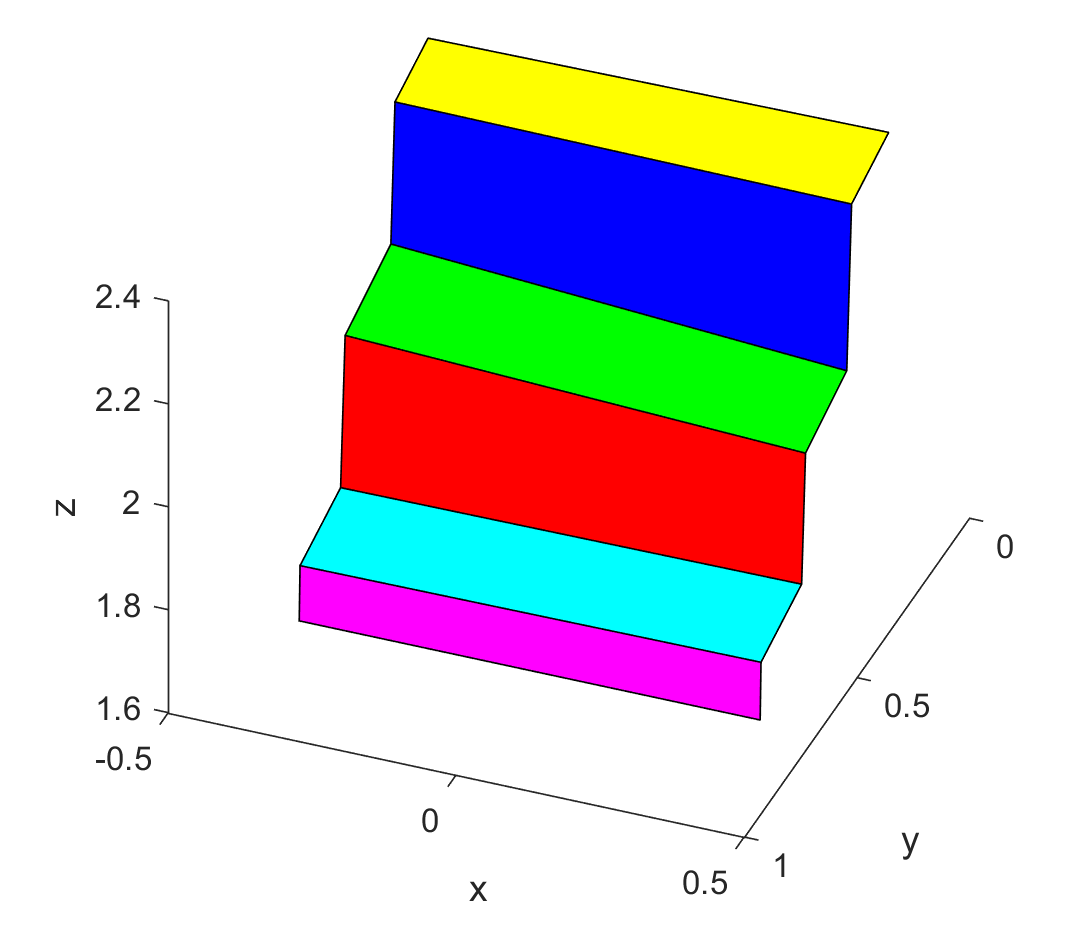
\includegraphics[width=2.5in]{Sections/Figures/polytope_example.png}
\caption{A polytope reconstruction of the image in Figure \ref{stereo-image-pair}, using the Contour Method (See Section \ref{contour-method}). The pink, red, and blue planes correspond to horizontal faces of the stairs. The light-blue, green, and yellow planes are vertical faces.}
\label{polytope-diagonal-contour}
\end{figure}

\begin{figure}[!h]
\centering
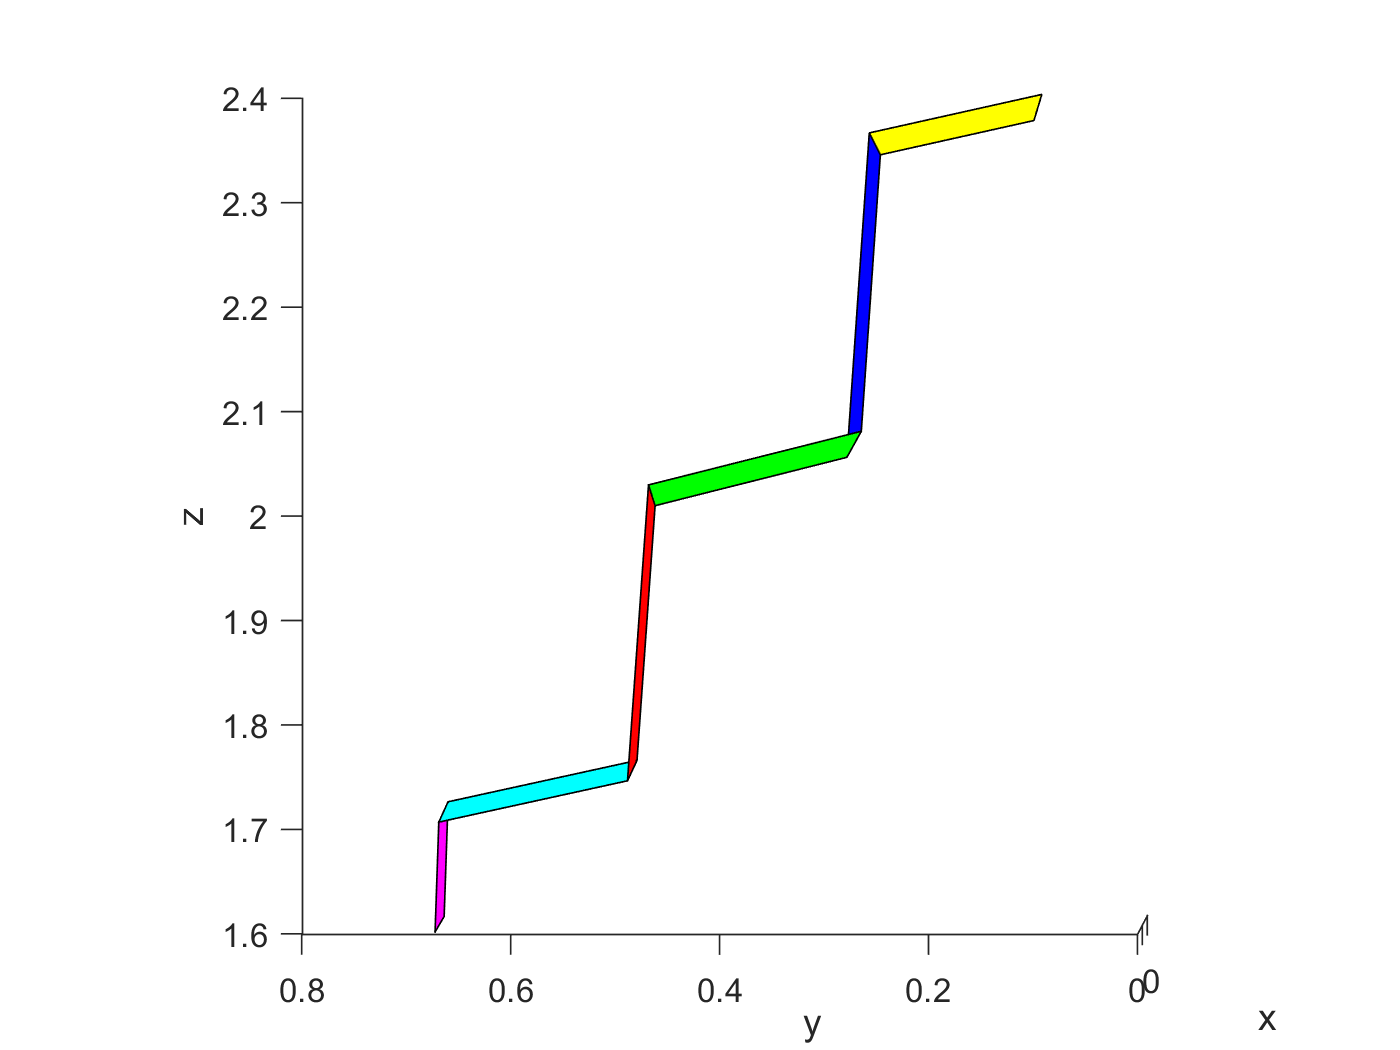
\includegraphics[width=3.1in]{Sections/Figures/polytope_sideview.png}
\caption{The polytope from Figure \ref{polytope-diagonal-contour} viewed from the side. The vertical faces of this polytope (light-blue, green, yellow) are very close to the groundtruth dimension of 20cm. Similarly, the remaining horizontal faces are close to their groundtruth dimension of 31cm.}
\label{polytope-sideview-contour}
\end{figure}

When using the Orientation Method in Section \ref{orient-method}, we use a sampling based approach to order planes. First, we sort all vertical planes based on their distance from the camera, then find the horizontal plane that is ``active'' between each pair of vertical planes. The ``active'' horizontal plane is the one that has the smallest average distance to a sample of points in the region between the vertical planes.


\begin{figure}[!h]
\centering
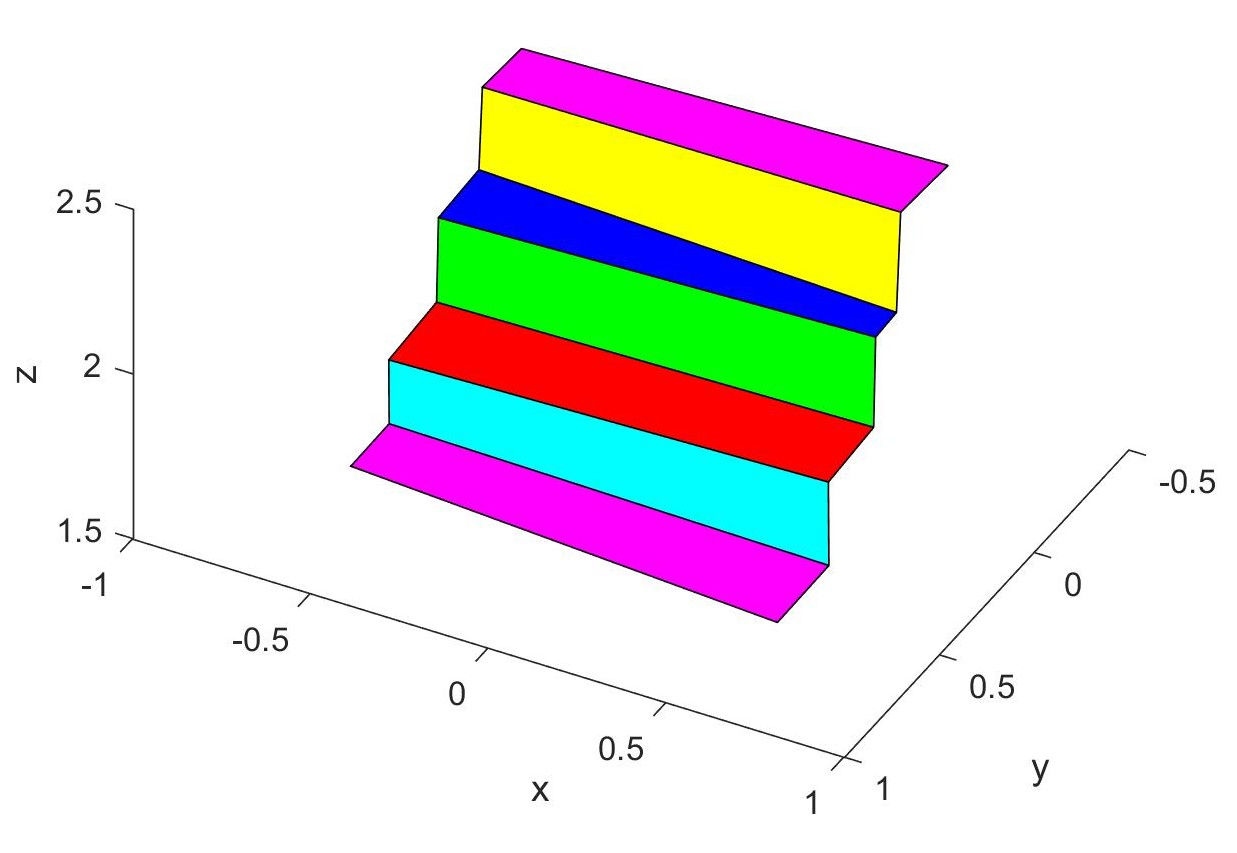
\includegraphics[width=3.3in]{Sections/Figures/polytope_diagonal_geom.jpg}
\caption{A polytope reconstruction of the image in Figure \ref{stereo-image-pair}, using the Orientation Method (See Section \ref{orient-method}). Here, the pink, red, and blue planes are vertical, and the light-blue, green, and yellow are horizontal. Because the orientation method is not limited by image contours, we are able to construct a polytope with more faces than in Figure \ref{polytope-diagonal-contour}}.
\label{polytope-diagonal-orient}
\end{figure}

\begin{figure}[!h]
\centering
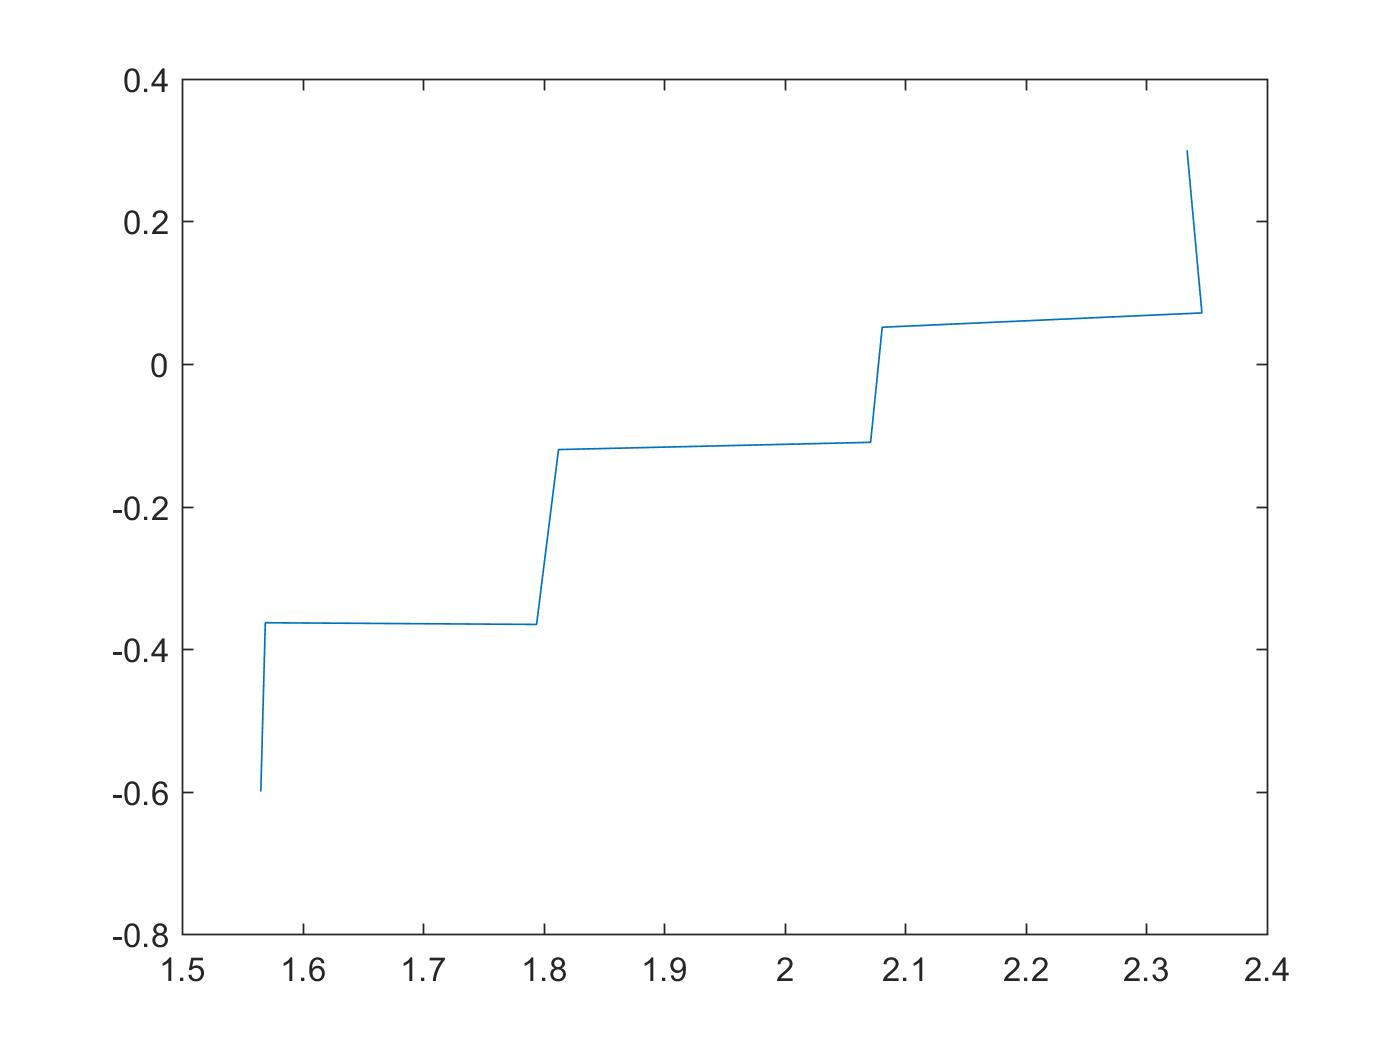
\includegraphics[width=3.3in]{Sections/Figures/geom_sideview_2d.jpg}
\caption{The polytope from Figure \ref{polytope-diagonal-orient} viewed from the side. Again, we see that vertical and horizontal planes are close to the groundtruth dimensions.}
\label{polytope-sideview-orient}
\end{figure}

Finally, once an ordering of planes has been established, we can compute lines of intersection between these planes, and obtain a set of vertices for the polytope. See Figures \ref{polytope-diagonal-contour} and \ref{polytope-diagonal-orient} for example reconstructions. See Figures \ref{polytope-sideview-contour} and \ref{polytope-sideview-orient} for a metric comparison of our reconstructions to groundtruth.


%!TEX root = ../egpaper_final.tex

\section{Results}


Since the robot previously used only reactive sensing of the environment this meant that the only way for the robot to sense obstacles and terrain was to physically interact with them. A robust reactive controller has been achieved and allows the robot to traverse highly unstructured terrains while remaining stable. However, while this makes the robot robust, there are situations where the terrain is not traversable easily without prior knowledge of the environment. Adding the vision system to the overall control system as an input to the path planning as seen in Figure \ref{fig:BD} will allow the robot to know if an obstacle is present, where it is, and its dimensions. Then it can decide how to modify its locomotion plan accordingly. For purposes of this demo the robot will attempt to detect the stair height and distance and modify its swing leg trajectory to place it on the stairs as its nominal swing foot height is lower than an average step.
\begin{figure}[!h]
\centering
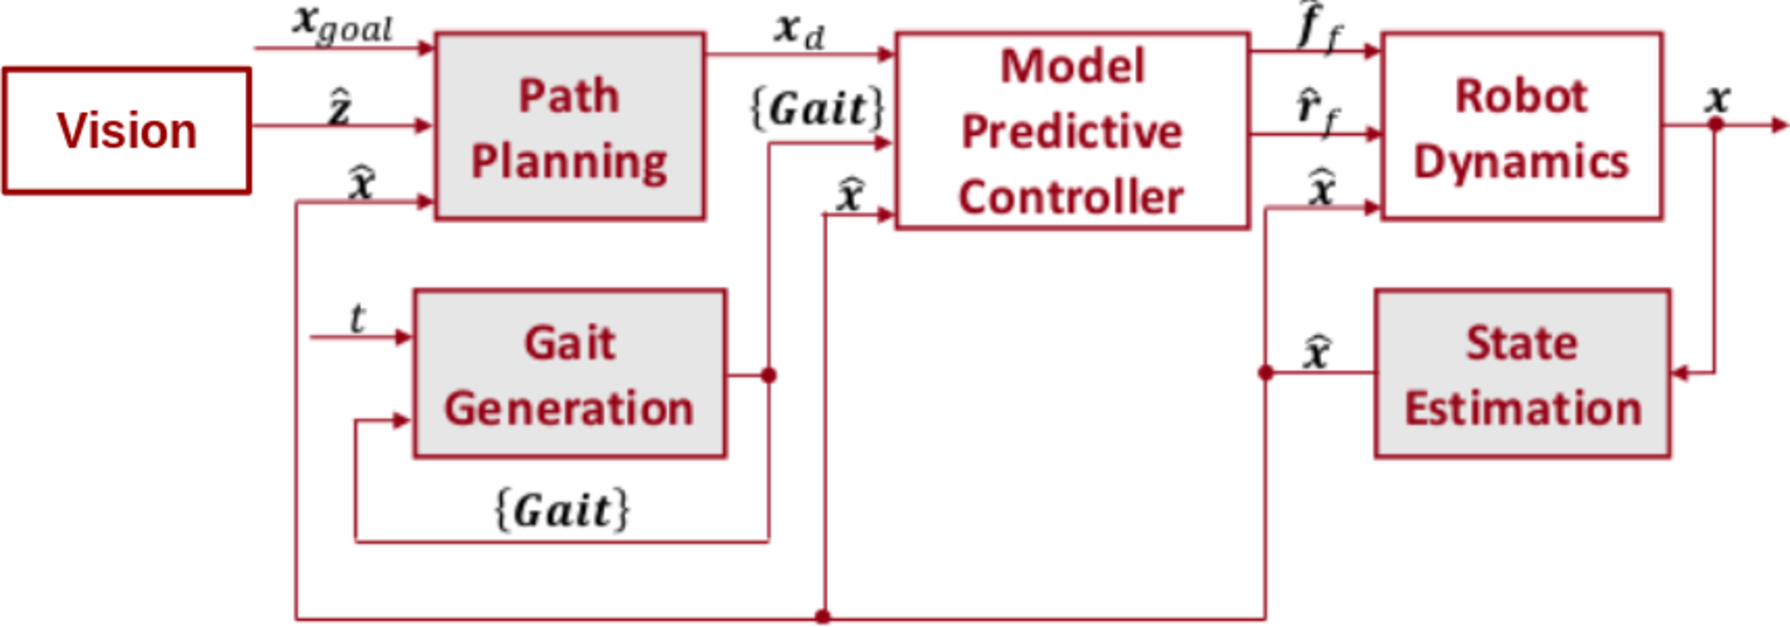
\includegraphics[width=\columnwidth]{Figures/BlockDiagram.pdf}
\caption{.}
\label{fig:BD}
\end{figure}


It is not enough to just find the dimensions of the object in front of the robot. This doesn't have any physical meaning to the robot until we find the relationship between the reconstructed object to the robot's coordinate frame. We take the points of interest of the object in the 3D camera frame, ${}^\mathcal{C}\bm{p}_o$, and apply the following transformation
\begin{equation}
{}^\mathcal{I}\bm{p}_o = {}^\mathcal{I}\bm{H}_\mathcal{C}{}^\mathcal{C}\bm{p}_o
\end{equation}
where ${}^\mathcal{I}\bm{H}_\mathcal{C}$ is the homogeneous transformation matrix between the camera frame and the Inertial frame. This allows the robot to know the distance and angle to the stairs relative to its body as seen in Figure \ref{fig:RSR}. With this, the robot now has knowledge about its environment without the need to physically interact with it. 
\begin{figure}[!h]
\centering
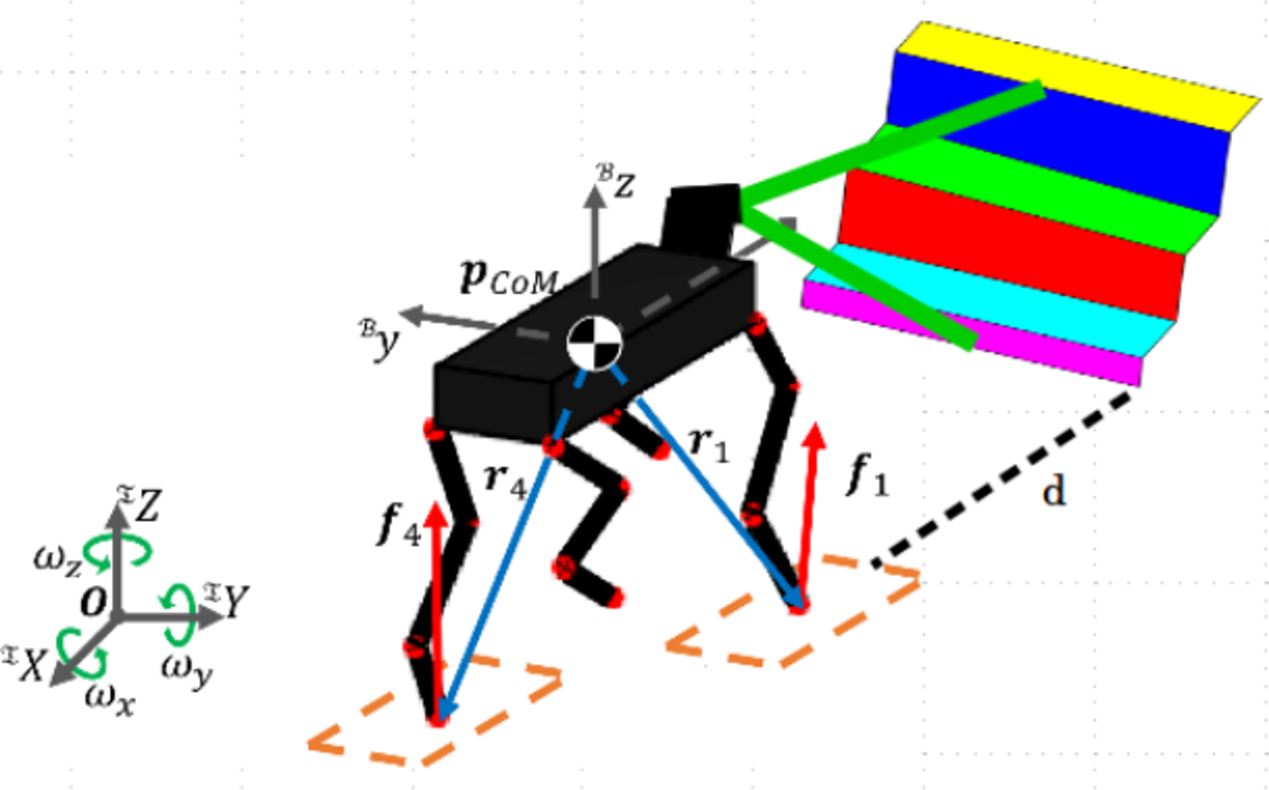
\includegraphics[width=\columnwidth]{Figures/RobotStairsRelation.pdf}
\caption{The robot must transform the coordinates of the stairs in the 3D reconstructed camera frame into the world frame in relation to the robot.}
\label{fig:RSR}
\end{figure}
With the robot holding an internal model of the environment with respect to its state, the path planner can adapt the nominal gait and foot placement trajectory to deal with the stairs at the detected height. The foot trajectory is modified when the robot's center of mass has traveled close enough to the detected stairs
\begin{equation}
({}^\Psi\bm{p}_{CoM,x} - {}^\Psi\bm{p}_{0,x}) < (d - d_{buffer})
\end{equation}
where ${}^\Psi\bm{p}_{CoM,x}$ is the yaw rotated CoM position ignoring pitch and roll effects, ${}^\Psi\bm{p}_{0,x}$ is the yaw rotated position at the last vision input, $d$ is the distance to the object at the detection time, and $d_{buffer}$ is a user defined buffer distance so that the robot begins lifting the legs slightly before the actual stair.


The vision system was successfully integrated with the robot software pipeline. Testing was first done in simulation where the webcams were used to detect the stairs and the robot was walked forward in simulation. The nominal trotting swing height for the leg trajectories is about 15 cm and the stair height was 21 cm. Therefore, the path planner made the decision to raise the height of the trajectory to about 30 cm, which was approximately 10 cm over the detected object height. When it reached the location of the 3D reconstructed stairs, the robot modified its foot trajectory appropriately. 

The pair of cameras was mounted on the physical robot and experiments were run with the real stair set on a treadmill. Figure \ref{fig:RS} shows the robot successfully climbing the stairs on its first attempt. With the terrain-blind controller, the most common failure mode was the robot being unable to get its leg over the stair and tripping. With the vision input, this was no longer the case as it knew how high to lift its leg and where to place the feet to aquire an adequate foothold.
\begin{figure}[!h]
\centering
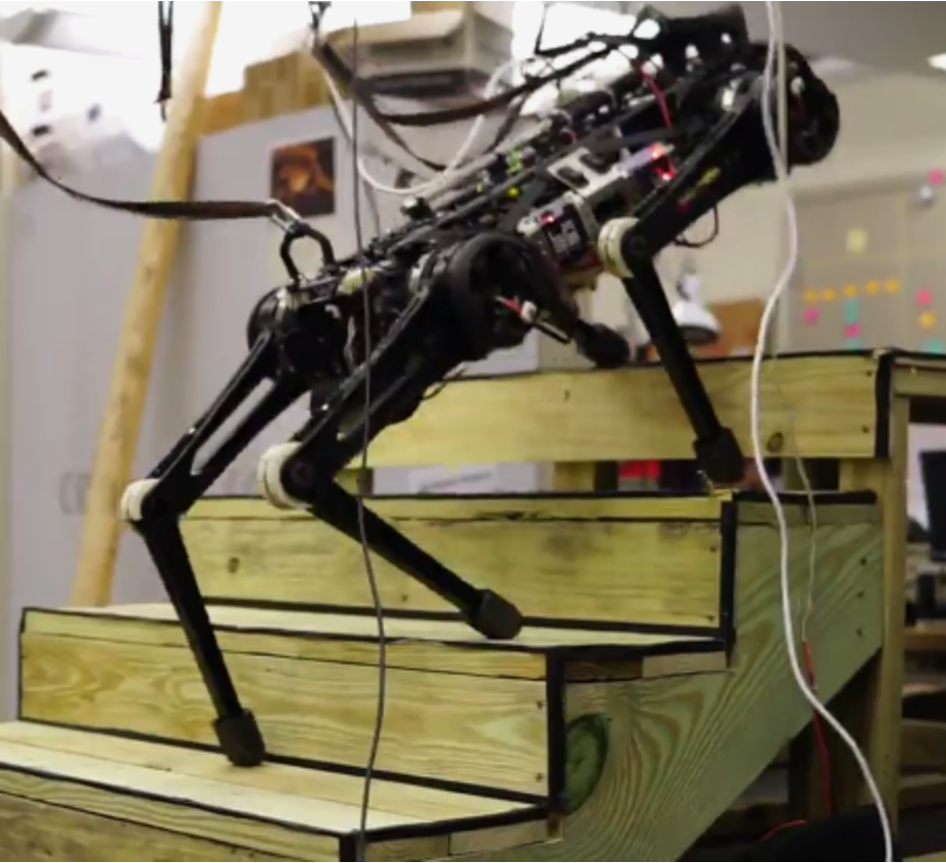
\includegraphics[width=0.85\columnwidth]{Figures/RobotStairs.pdf}
\caption{With the vision input, the robot is able to stably figure out how high to raise the feet in order to place them onto the stairs and successfully climb up.}
\label{fig:RS}
\end{figure}

%!TEX root = ../egpaper_final.tex

\section{Conclusion}

The presented vision system yielded promising results for use as a general terrain sensing solution for the MIT Cheetah robot during locomotion. Successful experiments showed its ability to accurately detect the location and dimensions of the stairs. Terrain information being provided to the robot helps the robot's path planning algorithms make better decisions when facing obstacles. Stability is improved as it anticipates contacts more accurately, rather than blindly relying on its reactive interactions with the physical world.

However, several practical limitations were noted when implementing the system. First and most importantly, the results were extremely sensitive to the camera calibration. As soon as the cameras moved slightly from the position they were calibrated in, the algorithms would return poor reconstructions. Similarly, if there was a slight lag between the frames that were taken on each camera, it would essentially act as if the cameras had moved with respect to each as the robot moves. The stereo algorithm also relies on having enough distinct features for disparity between the images. The work presented is a good first step towards robust robot vision, but more work would still be needed in the future. Overall, the system was successful in allowing the robot to climb stairs reliably under the experiment conditions.

%Abstract (10%)
%Introduction (10%)
%Related work (10%)
%Approach (and technical correctness) (20%)
%Experimental results (and technical correctness) (20%)
%Conclusion (6.667%)
%References (3.333%)
%Overall clarity of the report (10%)
%Reproducibility: can the work be reproduced from the information given in the report? (10%)

{\small
\bibliographystyle{ieee}
\bibliography{egbib}
}
%https://pdfs.semanticscholar.org/872e/9d71311cf9f00ec0ebc2c6b592c12a44d1f0.pdf

\end{document}
